\chapter{\Acrshort{ofdm} in GNU~Radio}\label{chap:ofdm-gnuradio}

This chapter is an extension of the \gls{ofdm} tutorial of the GNU~Radio Wiki\footnote{\url{https://wiki.gnuradio.org/index.php?title=Basic_OFDM_Tutorial}}.

% \begin{figure}[hbtp]
%     \centering
%     \begin{tikzpicture}[x=1.6cm,y=1.6cm]
%     \draw (0,0) rectangle +(1,0.4) node [midway] {A};
% \draw (1,0) rectangle +(1,0.4) node [midway] {A};
% \draw (-0.2,0) rectangle +(0.2,0.4) node [midway] {\rotatebox{90}{\tiny{CP}}};

% \foreach \i in {0,...,3} {
%   \draw (2+\i*2.2,0) rectangle +(0.2,0.4) node [midway] {\rotatebox{90}{\tiny{CP}}};
%   \draw (2.2+\i*2.2,0) rectangle +(2,0.4) node [midway] {Payload};
% }

% \draw [decorate, decoration={brace,amplitude=5pt,mirror}] (-0.2,-0.2) -- +(2.2,0) node [midway,below,yshift=-5pt] {Preamble};
% \draw [decorate, decoration={brace,amplitude=5pt,mirror}] (2,-0.2) -- +(4*2.2,0) node [midway,below,yshift=-5pt] {N OFDM Symbols};
% \end{tikzpicture}
% \end{figure}

\section{Conventions and Notations}\label{sec:ofdm-conventions}

\subsection{FFT Shifting}
In all cases where \gls{ofdm} symbols are passed between blocks, the default behaviour is to \gls{fft}-Shift these symbols, i.e., that the \gls{dc} carrier is in the middle (to be precise, it is on carrier floor(N/2) where $N$ is the \gls{fft} length and carrier indexing starts at $0$).
This means that when viewing \gls{ofdm} symbols, \gls{fft}-shifted symbols are in their natural order, i.e., as they appear in the pass band.

\subsection{Carrier Indexing}
Carriers are always index starting at the DC carrier, which has the index 0 (you usually don't want to occupy this carrier). The carriers right of the DC carrier (the ones at higher frequencies) are indexed with 1 through $N/2-1$ ($N$ being the FFT length again).

The carriers left of the DC carrier (with lower frequencies) can be indexed $-N/2$ through $-1$ or $N/2$ through $N-1$. Carrier indices $N-1$ and $-1$ are thus equivalent. \textit{The advantage of using negative carrier indices is that the FFT length can be changed without changing the carrier indexing.} For this reason, usage of negative carrier indices are recommended.

\subsection{Carrier and Symbol Allocation}
Many blocks require knowledge of which carriers are allocated, and whether they carry data or pilot symbols. GNU Radio blocks uses three objects for this, typically called \texttt{occupied\_carriers} (for the data symbols), \texttt{pilot\_carriers} and \texttt{pilot\_symbols} (for the pilot symbols). We advise you to follow these naming conventions.

Every one of these objects is a vector of vectors. \texttt{occupied\_carriers} and \texttt{pilot\_carriers} identify the position within \textit{a frame} where data and pilot symbols are stored, respectively.

\mintinline{python}{occupied_carriers[0]} identifies which carriers are occupied on the first OFDM symbol, \mintinline{python}{occupied_carriers[1]} does the same on the second OFDM symbol etc.

Here's an example:
\begin{minted}{python}
    occupied_carriers = ((-2, -1, 1, 3), (-3, -1, 1, 2))
    pilot_carriers = ((-3, 2), (-2, 3))
\end{minted}
Every OFDM symbol carries 4 data symbols. On the first OFDM symbol, they are on carriers -2, -1, 1 and 3. Carriers -3 and 2 are not used, so they are where the pilot symbols can be placed. On the second OFDM symbol, the occupied carriers are -3, -1, 1 and 2. The pilot symbols must thus be placed elsewhere, and are put on carriers -2 and 3.

If there are more symbols in the OFDM frame than the length of \mintinline{python}{occupied_carriers} or \mintinline{python}{pilot_carriers}, they wrap around (in this example, the third OFDM symbol uses the allocation in \mintinline{python}{occupied_carriers[0]}). We do not advise you to make use of this wrap around function, but rather recommend to properly define the carrier allocations.

But how are the pilot symbols set? This is a valid parameterization:

\begin{minted}{python}
    pilot_symbols = ((-1, 1j), (1, -1j), (-1, 1j), (-1j, 1))
\end{minted}
The position of these symbols are those in \mintinline{python}{pilot_carriers}. So on the first OFDM symbol, carrier -3 will transmit a -1, and carrier 2 will transmit a 1j. Note that \mintinline{python}{pilot_symbols} is longer than \mintinline{python}{pilot_carriers} in this example-- this is valid, the symbols in \mintinline{python}{pilot_symbols[2]} will be mapped according to \mintinline{python}{pilot_carriers[0]}. Again, we do not advise you to make use of wrap around functionality.

\section{Transmitting}

It is assumed that the input is a stream of complex scalars with a length tag, i.e., the transmitter will work on one frame at a time. An example flow graph can be found on: \url{https://github.com/gnuradio/gnuradio/blob/main/gr-digital/examples/ofdm/ofdm_loopback.grc}. This block is defined in \url{https://github.com/gnuradio/gnuradio/blob/main/gr-digital/python/digital/ofdm_txrx.py}.


\tikzset{
block/.style={
    minimum height=1cm,
     %maximum width=2cm,
      align=center,
      draw=black,
      fill=white,
      rectangle
    }
}




First, the input scalars are allocated according to the \texttt{OFDM Carrier Allocator} block. This sorts the incoming complex scalars onto OFDM carriers, and also places the pilot symbols onto the correct positions. There is also the option to pass OFDM symbols which are prepended in front of every frame (i.e. preamble symbols). These can be used for detection, synchronization, and channel estimation.

The carrier allocator outputs OFDM symbols (i.e. complex vectors of FFT length). These must be converted to time domain signals before continuing, which is why they are piped into th \texttt{FFT block}. Note that because all the OFDM symbols are treated in the shifted form, the IFFT block (i.e., reversed \texttt{FFT block}) must be shifting as well.

Finally, the cyclic prefix is added to the OFDM symbols, through the \texttt{OFDM Cyclic Prefixer}.

Next to this, the \texttt{OFDM Transmitter} block performs prepending two sync words, header, and payload modulation. For the remainder of the lab session, make use of the transmitter block, instead of separate blocks.

\begin{tikzpicture}[>=stealth, node distance=0.5cm and 0.5cm]
    % Nodes
    \node [coordinate] (start) {};
    
    
    \node [draw, block, right=of start] (crc) {CRC};
    \node [draw, block, above right=of crc] (headergen) {Header Gen};
    \node [draw, block, right=of headergen] (headermod) {Header Mod};
    \node [draw, block, below right=of headermod] (headerpayloadmux) {Header Payload Mux};
    
    \node [draw, block, below right=of crc] (payloadscrambler) {Payload Scrambler};
    \node [draw, block, right=of payloadscrambler] (payloadunpack) {Payload Unpack};
    \node [draw, block, right=of payloadunpack] (payloadmod) {Payload Mod};
    
    \node [draw, block, right=of headerpayloadmux] (allocator) {Allocator};

    \node [align=center, draw=none, above=of allocator] (sync) {Sync words};
    
    \node [draw, block, right=of allocator] (fft) {FFT};
    \node [draw, block, right=of fft] (cp) {CP};

    \node [coordinate, right=of cp] (end) {};
    
    % Arrows
    \draw[o->] (start) -- (crc);
    \draw[->] (crc) -- (headergen);
    \draw[->] (headergen) -- (headermod);
    \draw[->] (headermod) -- (headerpayloadmux);
    
    \draw[->] (crc) -- (payloadscrambler);
    \draw[->] (payloadscrambler) -- (payloadunpack);
    \draw[->] (payloadunpack) -- (payloadmod);
    \draw[->] (payloadmod) -- (headerpayloadmux);
    
    \draw[->] (headerpayloadmux) -- (allocator);
    \draw[->] (allocator) -- (fft);
    \draw[->] (fft) -- (cp);
    \draw[->o] (cp) -- (end);

    \draw[o->] (sync) -- (allocator);
    
\end{tikzpicture}

\subsection{OFDM Transmitter}

\subsubsection{Paramaters}

\begin{table}[]
    \centering
    \begin{tabular}{ll}
    \toprule
         FFT Length &  64\\
         Data subcarriers & 52 (-26 to 26)\\
         Pilot subcarriers (BPSK) & 4 (-21, -7, 7, 21)\\
         DC subcarrier & Null\\
         \Gls{bw} & \SI{20}{\mega\hertz}\\
         \Gls{obw} & \SI{16.6}{\mega\hertz}\\
         Subcarrier Frequency Spacing &	\SI{312.5}{\kilo\hertz}   (\SI{20}{\mega\hertz}/64)\\
         \bottomrule
    \end{tabular}
    \caption{802.11a OFDM}
    \label{tab:ofdm_params}
\end{table}

\begin{itemize}
    \item \textbf{FFT Length}\\
    The number of sub-carriers used per OFDM symbol. 
    \item \textbf{Cyclic Prefix Length}\\
    The maximum possible length of multi-paths in their time dispersion. Conventionally, the \gls{cp} length is equal to $\text{FFT}//4$.
    \item \textbf{Packet Length Tag Key}\\
    The name of the tag giving packet length at the input. This is propagated through the flow graph in order for all blocks to know how long each packet is.
    \item \textbf{Occupied Carriers}\\
    A vector of vectors describing which OFDM carriers are occupied with data symbols. \mintinline{python}{occupied_carriers[0]} identifies the carriers that are used for the first OFDM symbol, and so on. See~\cref{sec:ofdm-conventions} for details and conventions.
    \item \textbf{Pilot Carriers}\\
    A vector of vectors describing which OFDM carriers are occupied with pilot symbols. See~\cref{sec:ofdm-conventions} for details and conventions.
    \item \textbf{Pilot Symbols}\\
    A vector of vectors indicating the pilot symbols. See~\cref{sec:ofdm-conventions} for details and conventions.
    \item \textbf{Sync Word 1}\\
    The first sync preamble symbol. This has to be with zeros on alternating carriers, e.g., (0., 1.536, 0., -1.536, 0., ...). Used for fine and coarse frequency offset and timing estimation. Length of sync sequence must be the same as the value of FFT length. IF none is passed a random sync sequence is created for fine frequency offset and timing estimation. This is the first of typically two sync preamble symbols for the Schmidl \& Cox sync algorithm.
    The relevant feature of these symbols is that every second sub-carrier
    is zero. In the time domain, this results in two identical halves of
    the OFDM symbols. Symbols are always BPSK symbols. Carriers are scaled by sqrt(2) to keep total energy constant. Note, that the default sync word only contains symbols on the \mintinline{python}{occupied_carriers} indices.
    \item  \textbf{Sync Word 2}\\
    The second sync preamble symbol. This has to be filled entirely. Also used for coarse frequency offset and channel estimation. The length of sync sequence must be the same as the value of FFT length.  
    If None is used, it creates a random sync sequence for coarse frequency offset and channel estimation. This is the second of typically two sync preamble symbols for the Schmidl \& Cox sync algorithm. Symbols are always BPSK symbols. No scaling is applied, as all carriers (\mintinline{python}{occupied_carriers}) are used.
    \item \textbf{Header Modulation}\\
     It has two options:
    \begin{itemize}
        \item \acrfull{bpsk}
        \item  \acrfull{qpsk}
    \end{itemize}
    \item \textbf{Payload Modulation}\\
    It has three options:
    \begin{itemize}
        \item \acrfull{bpsk}
        \item  \acrfull{qpsk}
        \item  8-PSK (Eight Phase Shift Keying)
    \end{itemize}
\end{itemize}




\section{Receiver}

\subsection{Detection and Synchronization}
Before anything happens, an OFDM frame must be detected, the beginning of OFDM symbols must be identified, and frequency offset must be estimated. The effects of these synchronization and timing offsets are detailed in~\cref{sec:sysimp}. Here, we will focus on the Schmidl \& Cox method~\cite{650240}. This is implemented in the GNU~Radio block \textit{Schmidl \& Cox OFDM synch.}\footnote{\url{https://wiki.gnuradio.org/index.php/Schmidl_\%26_Cox_OFDM_synch.}}.

The evaluation of the coarse frequency offset is not done in this block. Also, the initial equalizer taps are not calculated here. This means the block performs a fine-grained frequency offset estimation and sync word detection, which you can use later for timing offset correction, i.e., start-of-frame detection.

\begin{figure}[htbp]
    \centering
    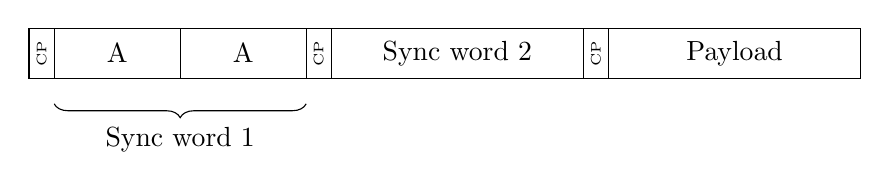
\begin{tikzpicture}[x=1.6cm,y=1.6cm]
    % SYN WORD 1
    \draw (0,0) rectangle +(1,0.4) node [midway] {A};
    \draw (1,0) rectangle +(1,0.4) node [midway] {A};
    \draw (-0.2,0) rectangle +(0.2,0.4) node [midway] {\rotatebox{90}{\tiny{CP}}};
    \draw [decorate, decoration={brace,amplitude=5pt,mirror}] (0.0,-0.2) -- +(2,0) node [midway,below,yshift=-5pt] {Sync word 1};

    % SYN WORD 2
    \draw (2.2,0) rectangle +(2,0.4) node [midway] {Sync word 2};
    \draw (2,0) rectangle +(0.2,0.4) node [midway] {\rotatebox{90}{\tiny{CP}}};

     % PAYLOAD
     \draw (4.4,0) rectangle +(2,0.4) node [midway] {Payload};
    \draw (4.2,0) rectangle +(0.2,0.4) node [midway] {\rotatebox{90}{\tiny{CP}}};
\end{tikzpicture}
\caption{Illustration of OFDM frame in GNU~Radio.}\label{fig:ofdm-frame-gnuradio}
\end{figure}

The OFDM frame is illustrated in~\cref{fig:ofdm-frame-gnuradio}. The first part comprises a \gls{cp} and the \texttt{sync word 1}, which in turn consists of two identical sequences. Often the \texttt{sync word 1} is constructed by only populating the carriers every second carrier, i.e., upsampling in the frequency domain, this yields two identical sequences in the time domain (A in~\cref{fig:ofdm-frame-gnuradio}). The sequences are designed such that their autocorrelation function has a sharp peak, being close to the dirac function. In order to thus find the start of frame, you need to find the sample offset where the correlation is highest. 

The correlation metric $P(d)$ for the received samples $z\left[n\right]$ can be written as,
\begin{equation}\label{eqOFDMpd} 
        P(d) = \sum_{i=0}^{N/2-1} z\left[\left(d+\frac{N}{2}\right)+ i\right]z^*\left[d+i\right].
\end{equation}
In other words, this function starts at index $d$ and computes the correlation of a sample at index $d+i$ with a sample $\frac{N}{2}$ samples further. Note, that the correlation is computed by taking the product of the conjugate of one sample with another sample. This function effectively takes two sequential windows of size $N/2$ and computes their correlation. If perfectly aligned, both windows contain the sequence $A$ and the correlation function yields the highest value. This method would work perfectly in ideal cases, but unfortunately, reality is never ideal. 

In real wireless systems, the signal will experience different attenuation at different time instances, resulting in a different magnitude of the received sequences ($A$), making the above referenced correlation method insufficient. To combat this, the metric $P(d)$ can be normalized by the energy of the samples within the correlation window.

In~\cite{650240}, the energy of the second part is computed only,
\begin{equation*} 
                R(d) = \sum_{i=0}^{N/2-1} \left|z\left[\left(d+\frac{N}{2}\right)+ i\right]\right|^2.
\end{equation*}
This differs from the computation in GNU~Radio which computes the energy of both halves. This avoids spurious detections at the end of a burst, when the energy level suddenly drops.

The new timing synchronization metric $M(d)$ is defined as,

\begin{equation}\label{eqOFDMmd} 
        M(d) = \frac{|P(d)|^2}{R(d)^2}.
\end{equation}

And the optimal timing instant is given as,
\begin{equation}\label{eqOFDMoptimalTiming} 
        \hat d = \max _{d} M(d) 
\end{equation}

GNU~Radio uses a plateau detector\footnote{\url{https://github.com/gnuradio/gnuradio/blob/main/gr-blocks/lib/plateau_detector_fb_impl.cc}} to estimate $\hat d$. This detector outputs a $1$ when the magnitude exceeds a configurable threshold for more than one sample. More extensive and complex detectors can be used, e.g., matched filtering.




